% AKULIN--KARLOV Fig.10.4. CP09 ink-vector source trace.
% Geometric source: cropped 1010 x 806 scan; real diagram in x=120..755.
% Four wavy amplitudes vs eight straight amplitudes; each dotted occurrence
% preserved, even when the physical index repeats. Crossing != vertex.
\documentclass[border=5pt]{standalone}
\usepackage{fontspec,unicode-math}
\setmainfont{Noto Serif}
\setmathfont{STIXTwoMath-Regular.otf}
\usepackage{tikz}
\usetikzlibrary{arrows.meta,decorations.pathmorphing,decorations.pathreplacing}
\tikzset{
 straight/.style={black,line width=.82pt,line cap=round},
 wavy/.style={black,line width=.84pt,decorate,
    decoration={snake,amplitude=.24mm,segment length=2.9mm,
    pre length=.8mm,post length=.6mm}},
 point/.style={black},
 grouping/.style={black,line width=.76pt,decorate,
    decoration={brace,amplitude=3.3pt}},
 grptext/.style={font=\fontsize{12.5}{15}\selectfont,inner sep=2pt},
 lab/.style={font=\fontsize{11.5}{13.8}\selectfont,inner sep=1.2pt}}
\begin{document}
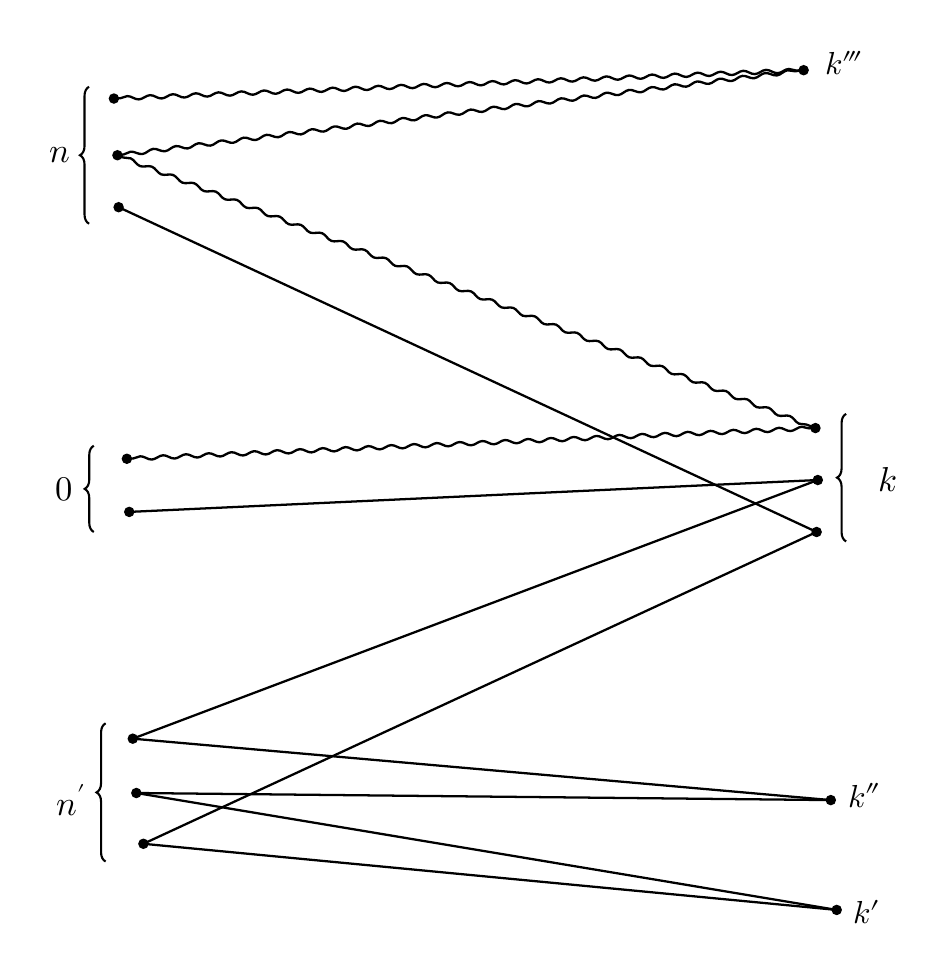
\begin{tikzpicture}[x=.015cm,y=-.015cm]
\path[use as bounding box] (55,19) rectangle (795,794);
% 14 inked occurrences: 3 n, 2 zero, 3 n', 3 k, k''', k'', k'.
\coordinate (n0) at (128,79);
\coordinate (n1) at (131,127);
\coordinate (n2) at (132,171);
\coordinate (z0) at (139,384);
\coordinate (z1) at (141,429);
\coordinate (np0) at (144,621);
\coordinate (np1) at (147,667);
\coordinate (np2) at (153,710);
\coordinate (kt) at (712,55);
\coordinate (k0) at (722,358);
\coordinate (k1) at (724,402);
\coordinate (k2) at (723,446);
\coordinate (kpp) at (735,673);
\coordinate (kp) at (740,766);
% Four WAVE factors, exactly paired at printed endpoints.
\draw[wavy] (n0)--(kt);
\draw[wavy] (n1)--(kt);
\draw[wavy] (n1)--(k0);
\draw[wavy] (z0)--(k0);
% Eight STRAIGHT factors; crossing points deliberately unmarked.
\draw[straight] (n2)--(k2);
\draw[straight] (z1)--(k1);
\draw[straight] (np0)--(k1);
\draw[straight] (np0)--(kpp);
\draw[straight] (np1)--(kpp);
\draw[straight] (np1)--(kp);
\draw[straight] (np2)--(k2);
\draw[straight] (np2)--(kp);
\foreach \p in {n0,n1,n2,z0,z1,np0,np1,np2,kt,k0,k1,k2,kpp,kp}{
   \fill[point] (\p) circle (1.9pt);
}
% Braces give index groups, not graph edges.
\draw[grouping] (107,185)--(107,69);
\draw[grouping] (111,446)--(111,373);
\draw[grouping] (121,725)--(121,608);
\draw[grouping] (748,454)--(748,346);
\node[grptext,anchor=east] at (96,127) {$n$};
\node[grptext,anchor=east] at (98,410) {$0$};
\node[grptext,anchor=east] at (110,673) {$n'$};
\node[grptext,anchor=west] at (770,402) {$k$};
\node[lab,anchor=west] at (727,49) {$k'''$};
\node[lab,anchor=west] at (747,669) {$k''$};
\node[lab,anchor=west] at (751,768) {$k'$};
\end{tikzpicture}
\end{document}
